\documentclass[conference,a4paper]{IEEEtran}

\usepackage{iftex}
\ifPDFTeX
  \usepackage[T5]{fontenc}
  \usepackage[utf8]{inputenc}
  \usepackage[vietnamese]{babel}
  \usepackage{lmodern}
\else
  \usepackage{fontspec}
  \setmainfont{DejaVu Serif}
  \setsansfont{DejaVu Sans}
  \setmonofont{DejaVu Sans Mono}
\fi
\usepackage{booktabs}
\usepackage{array}
\usepackage{url}
\usepackage{microtype}
\usepackage{graphicx}
\usepackage{placeins}

\newcommand{\authorname}{Bùi Huyền Mi}
\newcommand{\mentorname}{Bùi Lê Huy}
\newcommand{\mentorunit}{VTIT}
\newcommand{\mentoremail}{huybuile2004@gmail.com}
\newcommand{\code}[1]{\texttt{#1}}
\renewcommand{\refname}{TÀI LIỆU THAM KHẢO}

% Xoá \screenshotplaceholder và thay bằng
% \includegraphics[width=\linewidth]{đường/dẫn/anh.png} khi đã có ảnh thật.
\newcommand{\screenshotplaceholder}[1]{%
  \fbox{\parbox[c][3.2cm][c]{0.94\linewidth}{\centering\footnotesize CHỖ CHÈN ẢNH\\[3pt]#1}}%
}

\title{XÂY DỰNG NỀN TẢNG LAKEHOUSE
THEO DÕI THỊ TRƯỜNG CHỨNG KHOÁN HOSE}

\author{
\IEEEauthorblockN{\authorname, \mentorname\textsuperscript{1}}
\IEEEauthorblockA{\textsuperscript{1}\mentorunit\\
Email: \mentoremail}
}

\begin{document}
\maketitle

\begin{abstract}
Báo cáo trình bày quá trình xây dựng một nền tảng dữ liệu cho thị trường chứng khoán HOSE, hợp nhất giá cổ phiếu, hồ sơ doanh nghiệp, chỉ số thị trường, tin tức và giao dịch trong phiên vào cùng một hệ thống. Dữ liệu được tổ chức qua ba tầng Bronze--Silver--Gold, kết hợp một pipeline xử lý theo lô chạy hằng ngày với một pipeline xử lý dòng cho dữ liệu thời gian thực, cùng một pipeline riêng thu thập và phân tích cảm xúc tin tức theo chu kỳ ngắn. Toàn bộ quá trình thu thập, chuẩn hóa, kiểm tra chất lượng và cảnh báo được điều phối tự động, có khả năng chạy lại khi gặp lỗi. Kết quả kiểm chứng cho thấy dữ liệu nhất quán giữa các tầng, đồng thời báo cáo cũng chỉ ra một số hạn chế thực tế còn tồn tại và hướng hoàn thiện tiếp theo.
\end{abstract}

\begin{IEEEkeywords}
Lakehouse, HOSE, Airflow, MinIO, ClickHouse, Kafka, dbt, VWAP, data quality.
\end{IEEEkeywords}

\section{GIỚI THIỆU CHUNG}

Dữ liệu thị trường chứng khoán có nhiều nhịp cập nhật khác nhau: giá và chỉ báo kỹ thuật theo phiên, hồ sơ doanh nghiệp thay đổi chậm, tin tức trong ngày, còn tick khớp lệnh và nến phút phát sinh liên tục trong giờ giao dịch. Chỉ lưu batch thì không phản ánh được diễn biến trong phiên; chỉ ưu tiên streaming thì thiếu lịch sử ổn định để tính toán và tái xử lý. Bài toán đặt ra là một nền tảng vừa bảo toàn dữ liệu gốc, vừa truy vấn nhanh, vừa nói rõ dữ liệu nào là cuối ngày và dữ liệu nào đang cập nhật.

Phạm vi hiện tại gồm 404 mã cổ phiếu HOSE, VNINDEX và VN30. Mục tiêu là hợp nhất dữ liệu có tần suất khác nhau; chuẩn hóa qua Bronze--Silver--Gold; tự động hóa thu thập và kiểm tra chất lượng; cung cấp giá cuối ngày (end-of-day, EOD), nến một phút, VWAP, chỉ báo kỹ thuật, cảm xúc tin tức, watchlist và cảnh báo. Điểm nổi bật là tách lớp lưu trữ khỏi lớp phục vụ, duy trì hai luồng thời gian thực độc lập (VWAP từ tick khớp lệnh và nến từ kênh DNSE riêng) để đối chiếu, đồng thời hỗ trợ cảnh báo theo sự kiện cắt ngưỡng (\emph{threshold crossing}) thay vì gửi lặp lại khi chỉ báo vẫn nằm ngoài ngưỡng.

Các đóng góp chính gồm thiết kế mô hình dữ liệu ba tầng, xây dựng hai DAG Airflow, triển khai luồng Kafka--ClickHouse cho VWAP và nến phút, xây dựng bộ đối soát liên tầng, tích hợp phân loại cảm xúc tin tức, phát triển API/dashboard và cơ chế cảnh báo đa kênh. Toàn bộ thành phần được đóng gói để có thể tái lập trên môi trường Docker Compose.

Mã nguồn và hướng dẫn triển khai được công bố tại \url{https://github.com/mihuyen/DataEngineerVDT}.

\section{NỘI DUNG VÀ PHƯƠNG PHÁP}

\subsection{Kiến trúc tổng thể}

Hạ tầng được triển khai bằng Docker Compose và chia thành bốn nhóm. MinIO, ClickHouse và PostgreSQL đảm nhiệm lưu trữ; Airflow điều phối công việc; Kafka, ZooKeeper và các DNSE producer xử lý dữ liệu trong phiên; FastAPI, React, Superset, Grafana, Alert Engine và dịch vụ NLP đảm nhiệm phục vụ và giám sát. Parquet trên MinIO lưu dữ liệu có thể truy vết và tái xử lý; ClickHouse tối ưu truy vấn phân tích; PostgreSQL lưu dữ liệu ứng dụng thay đổi thường xuyên như watchlist và quy tắc cảnh báo. dbt được gọi từ Airflow để xây dựng mart chỉ báo kỹ thuật.

\begin{figure*}[t]
  \centering
  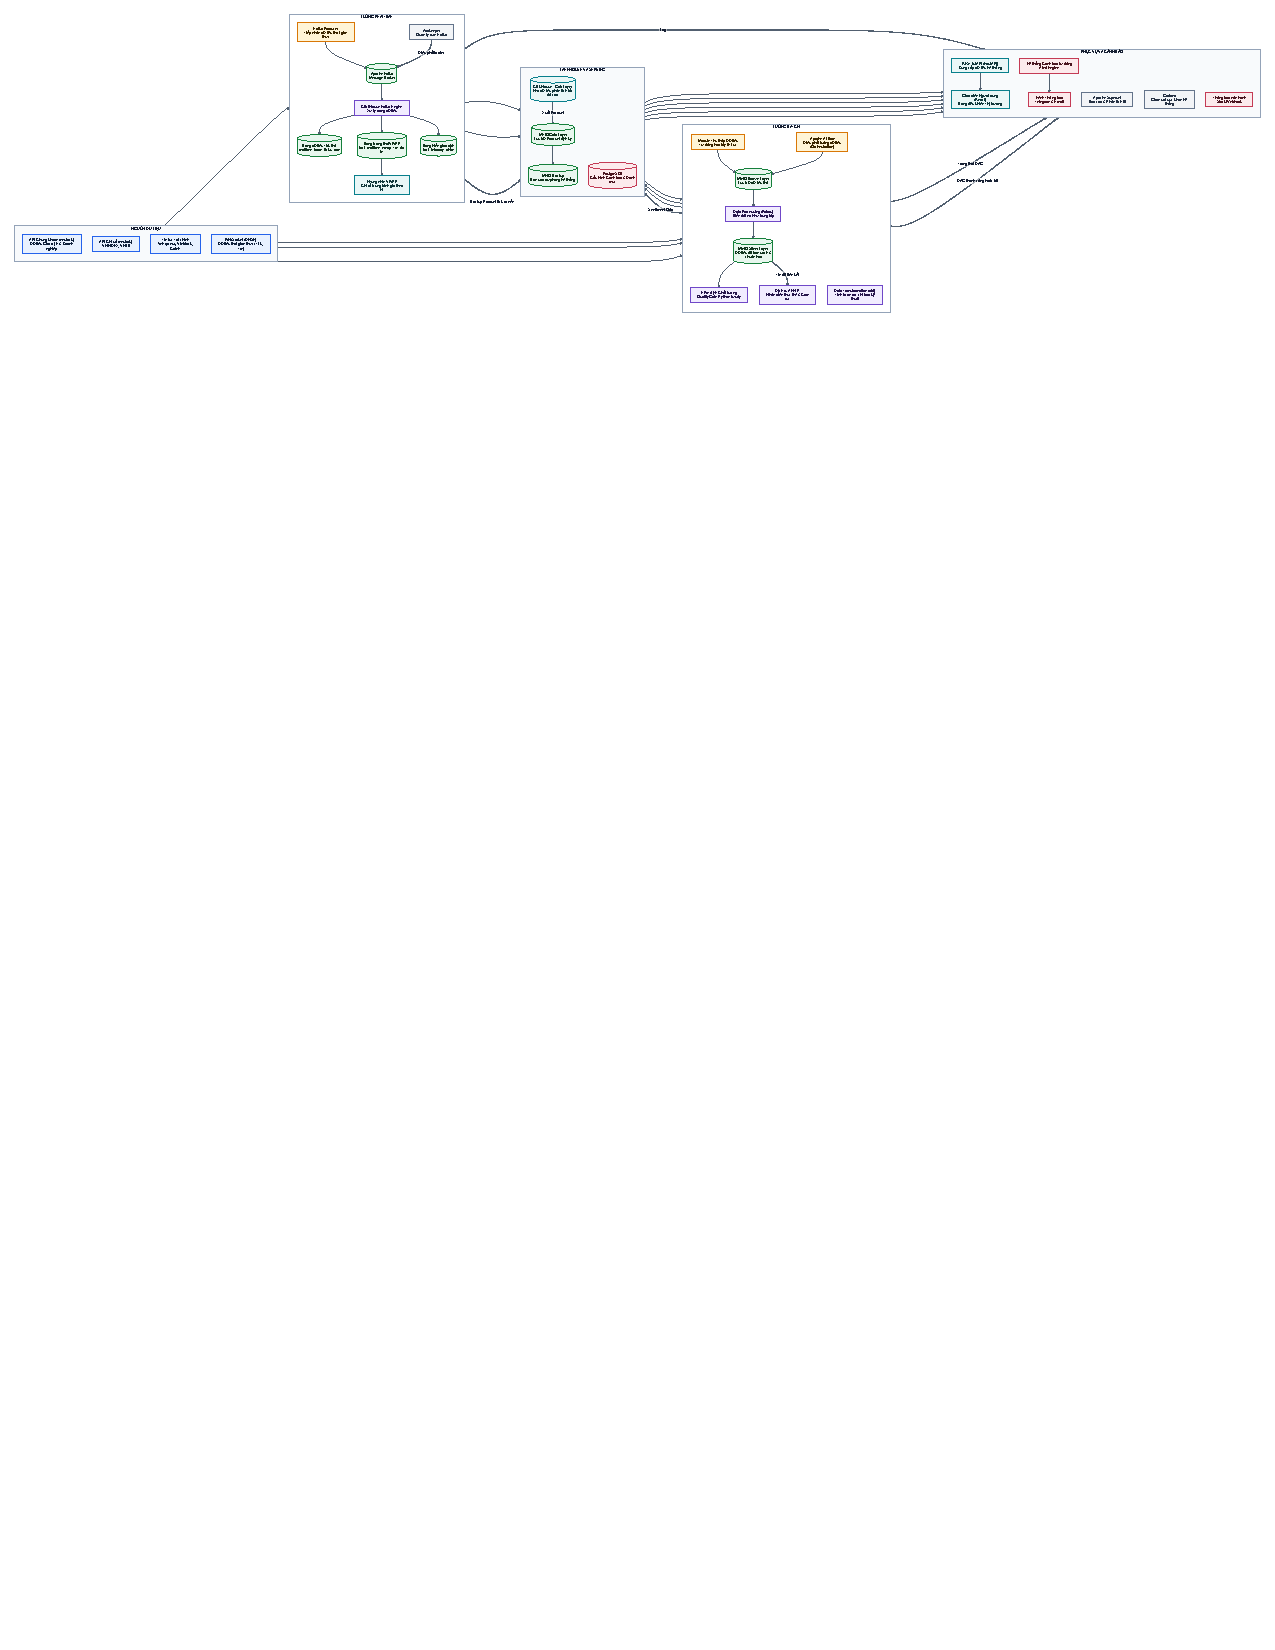
\includegraphics[width=0.92\textwidth]{../docs/architecture/system_architecture.pdf}
  \caption{Kiến trúc tổng thể: nguồn dữ liệu, luồng batch, luồng streaming, lớp serving và tiêu thụ.}
  \label{fig:architecture}
\end{figure*}

Theo Armbrust \textit{et al.}~\cite{lakehouse}, kiến trúc Lakehouse kết hợp khả năng lưu trữ linh hoạt của Data Lake với quản trị dữ liệu và hiệu năng truy vấn của Data Warehouse. Một triển khai đầy đủ thường có table format như Delta Lake, Apache Iceberg hoặc Apache Hudi để cung cấp giao dịch ACID, tiến hóa lược đồ (\emph{schema evolution}) và truy vấn phiên bản dữ liệu (\emph{time travel}). Hệ thống hiện áp dụng kiến trúc Medallion và tách lớp lưu trữ khỏi lớp phục vụ, nhưng Parquet trên MinIO chưa có table format. Vì vậy, báo cáo sử dụng thuật ngữ \emph{nền tảng theo kiến trúc Lakehouse}; Apache Iceberg là hướng hoàn thiện được trình bày tại Mục~\ref{sec:future}.

\subsection{Nguồn dữ liệu}

Bảng~\ref{tab:sources} tổng hợp bốn nguồn: ba nguồn đầu vận hành theo lô, riêng DNSE theo dòng liên tục trong giờ giao dịch -- lý do hệ thống cần hai kiến trúc thu thập song song.

\textbf{OHLCV và danh sách niêm yết.} Danh sách mã và hồ sơ doanh nghiệp được lấy qua thư viện vnstock với nguồn KBS; giá OHLCV sử dụng nguồn VCI. Mỗi yêu cầu trả về giá mở cửa, cao nhất, thấp nhất, đóng cửa và khối lượng. Tùy chọn \code{--skip-existing} giúp lần chạy lại bỏ qua phân vùng đã có. Tại Silver, pipeline chuẩn hóa kiểu ngày và số, loại bản ghi thiếu khóa, kiểm tra quan hệ \code{high >= open, close, low} và chỉ giữ mã HOSE.

\textbf{Chỉ số thị trường.} VNINDEX và VN30 cũng lấy qua vnstock (VCI), khai báo tường minh trong cấu hình nguồn; Silver chỉ chấp nhận đúng hai mã này. Khi lên Gold, pipeline nối với \code{dim\_index}, tính biến động điểm, SMA20, RSI14 và độ rộng thị trường (số mã tăng/giảm/đứng giá trong HOSE, VN30 dùng danh sách thành phần tại thời điểm chạy).

\textbf{Tin tức.} DAG \code{news\_crawl\_5m} chạy mỗi 5 phút, độc lập với DAG batch 18:00. Pipeline thu thập bài từ VnExpress, Vietstock và CafeF; URL registry lưu URL chuẩn hóa để chỉ tải bài mới. Silver làm sạch nội dung và loại trùng. Bước liên kết thực thể (\emph{entity linking}) sử dụng mã cổ phiếu, tên doanh nghiệp và ngữ cảnh xuất hiện để gắn một bài với một hoặc nhiều mã HOSE. Dịch vụ PhoBERT phân loại ba nhãn tích cực, trung lập và tiêu cực; mỗi dự đoán lưu điểm, độ tin cậy, phiên bản mô hình và thời điểm suy luận trong \code{fact\_news\_sentiment\_detail}. Bảng \code{fact\_news\_sentiment\_daily} sau đó tổng hợp theo \code{ticker + news\_date}.

\begin{table}[t]
\caption{Nguồn dữ liệu và đích phục vụ}
\label{tab:sources}
\centering
\scriptsize
\begin{tabular}{p{1.5cm}p{2.3cm}p{3.2cm}}
\toprule
\textbf{Nguồn} & \textbf{Nhịp cập nhật} & \textbf{Nội dung và đích} \\
\midrule
KBS (vnstock) & Sau giờ giao dịch & Danh sách HOSE, hồ sơ doanh nghiệp \\
VCI (vnstock) & Sau giờ giao dịch & OHLCV ngày, VNINDEX, VN30 \\
Báo chí & Theo chu kỳ crawl & Tin tức, cảm xúc thị trường \\
DNSE WebSocket & Trong giờ giao dịch & Tick khớp lệnh, nến 1 phút \\
\bottomrule
\end{tabular}
\end{table}

\subsection{Tổ chức Bronze--Silver--Gold}

Bronze giữ dữ liệu gần nguyên trạng và bổ sung thông tin về nguồn, thời điểm thu thập. OHLCV được phân vùng theo \code{year/month/day}, trong đó toàn bộ mã của một ngày được gộp vào một file Parquet. Nếu chia tiếp theo ticker, mỗi ngày sẽ phát sinh hàng trăm file nhỏ, làm tăng chi phí liệt kê và mở đối tượng trên MinIO (\emph{small-file problem}). Silver gộp OHLCV theo \code{year/month}. Khi truy vấn một mã, hệ thống phải đọc rồi lọc dữ liệu của tháng tương ứng; đổi lại, số file giảm đáng kể và Parquet vẫn hỗ trợ chỉ đọc các cột cần thiết (\emph{column pruning}).

Gold sử dụng mô hình sao (\emph{star schema}) với bốn bảng chiều: \code{dim\_date}, \code{dim\_stock}, \code{dim\_sector}, \code{dim\_index}. Các bảng sự kiện lưu giá ngày, chỉ số, nến phút, VWAP, cảm xúc tin tức và cảnh báo. Mỗi bảng có mức chi tiết bản ghi (\emph{grain}) và khóa sắp xếp phù hợp với truy vấn chính. Một lỗi ở Gold có thể truy ngược về bản ghi Silver và phân vùng Bronze tương ứng mà không cần thu thập lại toàn bộ dữ liệu.

\begin{table}[t]
\caption{Data contract qua ba tầng}
\label{tab:layers}
\centering
\scriptsize
\begin{tabular}{p{1.0cm}p{2.7cm}p{3.3cm}}
\toprule
\textbf{Tầng} & \textbf{Trách nhiệm} & \textbf{Kiểm soát chính} \\
\midrule
Bronze & Bảo toàn dữ liệu nguồn và metadata & Nguồn, thời điểm, phân vùng \\
Silver & Chuẩn hóa lược đồ và khóa nghiệp vụ & Giá trị thiếu, miền hợp lệ, tính duy nhất \\
Gold & Mô hình phục vụ và chỉ báo & Khóa chiều/sự kiện, độ tươi \\
\bottomrule
\end{tabular}
\end{table}

\begin{figure*}[t]
  \centering
  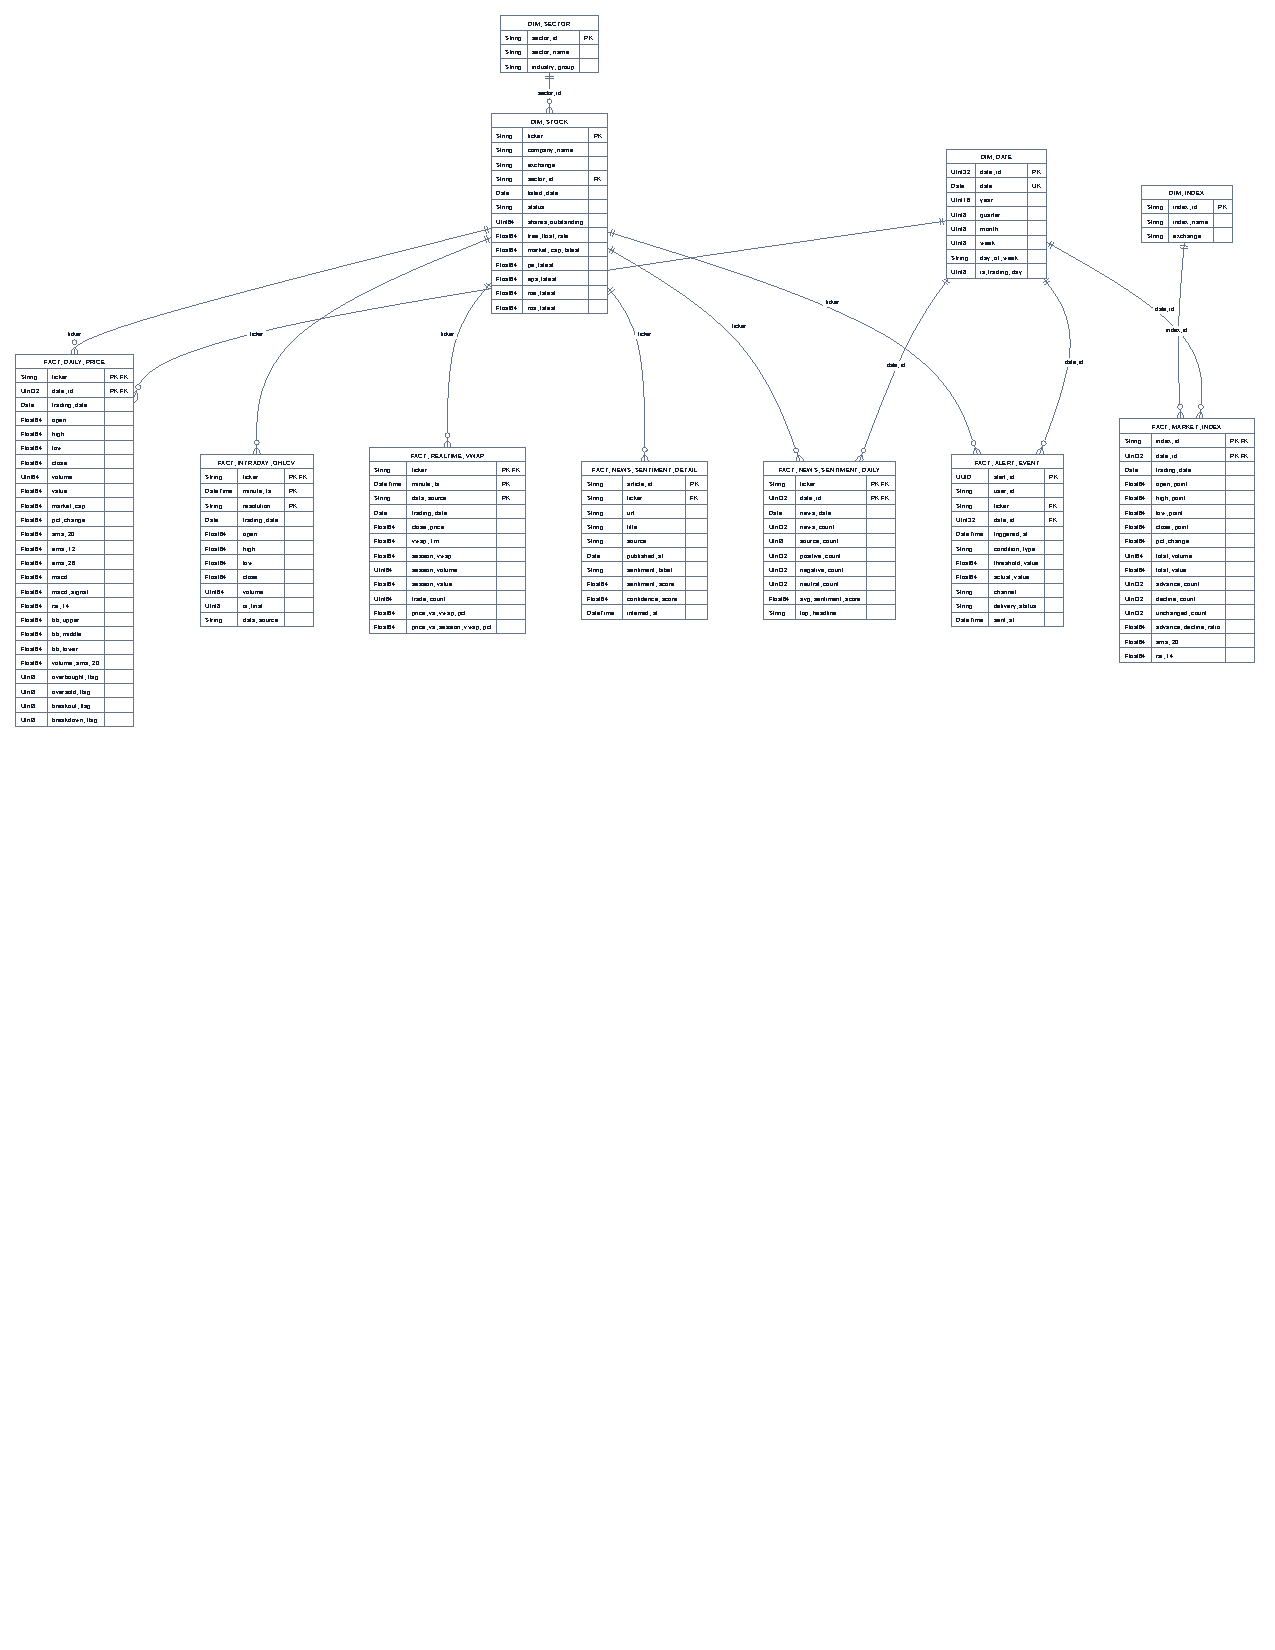
\includegraphics[width=0.92\textwidth]{../docs/architecture/gold_star_schema.pdf}
  \caption{Mô hình sao tầng Gold: bốn bảng chiều dùng chung và các bảng sự kiện có mức chi tiết riêng.}
  \label{fig:schema}
\end{figure*}

\subsection{Pipeline theo lô và dbt}

DAG \code{stock\_lakehouse\_daily} chạy lúc 18:00 từ thứ Hai đến thứ Sáu. Ba nhánh giá, hồ sơ doanh nghiệp và chỉ số chạy song song, sau đó lần lượt chuẩn hóa Silver, kiểm tra chất lượng, nạp Gold, đối soát, chạy dbt, xuất Parquet và kiểm tra cảnh báo. DAG này không thu thập, suy luận hoặc nạp lại dữ liệu news. DAG \code{news\_crawl\_5m} là chủ sở hữu duy nhất của luồng tin tức và chạy theo chu kỳ 5 phút trong suốt 24 giờ.

dbt~\cite{dbt} được sử dụng cho phép biến đổi trong ClickHouse~\cite{clickhouse}, chủ yếu tính chỉ báo bằng hàm cửa sổ SQL (\emph{window function}). Kiểm tra chất lượng liên tầng được viết bằng Python vì \code{dbt test} chủ yếu kiểm tra quan hệ trong dự án dbt, trong khi hệ thống cần phát hiện mất bản ghi từ Bronze sang Silver và sai khác khóa từ Silver sang Gold. Loader Gold bảo vệ các bảng do dịch vụ thời gian thực sở hữu; các bảng theo lô sử dụng mốc dữ liệu đã nạp (\emph{watermark}) và chỉ ghi lại phân vùng tháng bị ảnh hưởng.

\subsection{Pipeline thời gian thực và VWAP}

Luồng thời gian thực đi từ DNSE WebSocket qua producer chuẩn hóa đến Kafka~\cite{kafka}. ClickHouse đọc Kafka bằng Kafka Engine. Materialized View thứ nhất ghi tick vào \code{realtime\_trade\_ticks\_raw}; Materialized View thứ hai tổng hợp tick thành trạng thái theo phút trong \code{fact\_realtime\_vwap\_1m\_state}. Bảng này dùng \code{AggregatingMergeTree} để gộp các trạng thái tổng hợp khi tick của cùng một phút đến ở nhiều đợt khác nhau. \code{fact\_realtime\_vwap} là một view truy vấn các trạng thái đã gộp và tính VWAP lũy kế trong phiên bằng hàm cửa sổ. Nến một phút được ghi vào \code{fact\_intraday\_ohlcv} dùng \code{ReplacingMergeTree(ingested\_at)}; khi DNSE gửi lại một nến đã hiệu chỉnh, phiên bản có thời điểm nạp mới hơn được giữ lại.

Các bảng vật lý thời gian thực đều có thời gian lưu (\code{TTL}) 30 ngày vì chỉ phục vụ nhu cầu xem trong phiên. Tiến trình thu thập đồng thời ghi Parquet lên MinIO để giữ dữ liệu gốc sau khi ClickHouse tự xóa dữ liệu hết hạn.

\subsection{Cảnh báo và chất lượng dữ liệu}

Quy tắc cảnh báo được lưu trong PostgreSQL, còn sự kiện đã kích hoạt được ghi vào ClickHouse. Hệ thống hỗ trợ 14 điều kiện, gồm ngưỡng tĩnh, dừng lỗ/chốt lời và cắt ngưỡng RSI hoặc VWAP. Bảng \code{fact\_alert\_rule\_state} lưu giá trị của chu kỳ trước để chỉ phát cảnh báo tại thời điểm cắt ngưỡng. Khoảng nghỉ giữa hai cảnh báo (\emph{cooldown}) và cơ chế gộp thông báo (\emph{digest}) giúp giảm gửi lặp. Airflow~\cite{airflow} gửi Slack khi tác vụ hết số lần thử lại hoặc khi DAG hoàn tất.

Khung chất lượng tham chiếu các chiều phổ biến trong DAMA-DMBOK: tính đầy đủ (\emph{completeness}), tính duy nhất (\emph{uniqueness}), tính hợp lệ (\emph{validity}), độ chính xác (\emph{accuracy}), tính nhất quán (\emph{consistency}) và tính kịp thời (\emph{timeliness}). Bronze chỉ kiểm tra khả năng đọc và metadata để giữ bằng chứng nguồn. Silver kiểm tra giá trị thiếu, miền giá trị OHLC và khóa duy nhất. Đối soát Bronze--Silver--Gold kiểm tra cả số lượng lẫn tập khóa nghiệp vụ; nhờ đó vẫn phát hiện được trường hợp hai tầng có cùng số dòng nhưng khác ticker hoặc ngày giao dịch. Độ tươi được tính theo ngày làm việc. Kiểm tra realtime mang tính giám sát và không chặn pipeline, vì dữ liệu trong phiên có thể tạm thời thiếu hoặc đến trễ. Độ chính xác tuyệt đối vẫn cần nguồn tham chiếu độc lập và chưa được tự động hóa.

Về khả năng quan sát (\emph{observability}), hệ thống đã có số đo vận hành và nhật ký theo tác vụ. Grafana hiển thị độ trễ, độ tươi và số bản ghi từ ClickHouse. Tuy nhiên, hệ thống chưa có truy vết phân tán (\emph{distributed tracing}) để theo dõi một tick xuyên suốt WebSocket--Kafka--Materialized View--API.

\section{KẾT QUẢ THỰC HIỆN}

Các số liệu trong Bảng~\ref{tab:results} được chụp tại ngày 06/07/2026 bằng truy vấn trực tiếp trên ClickHouse; số dòng được tính bằng \code{count()} thay vì metadata của các part chưa hợp nhất.

\begin{table}[t]
\caption{Kết quả dữ liệu và kiểm chứng}
\label{tab:results}
\centering
\scriptsize
\begin{tabular}{p{3.1cm}p{1.2cm}p{2.4cm}}
\toprule
\textbf{Đối tượng} & \textbf{Số lượng} & \textbf{Ghi chú} \\
\midrule
Mã cổ phiếu HOSE & 404 & Không gồm HNX/UPCOM \\
\code{fact\_daily\_price} & 14.948 & 171 ngày giao dịch \\
\code{fact\_daily\_price\_indicators} & 14.947 & Mart dbt dạng tăng dần \\
\code{fact\_market\_index} & 78 & VNINDEX và VN30 \\
\code{fact\_intraday\_ohlcv} & 27.973 & TTL 30 ngày \\
\code{fact\_alert\_event} & 887 & 292 lần gửi thành công \\
\code{fact\_news\_sentiment\_detail} & 1.895 & 1.169 bài, 204 mã \\
\code{fact\_news\_sentiment\_daily} & 1.207 & Tổng hợp mã--ngày \\
Airflow & 2 DAG & Batch ngày và news 5 phút \\
Reconciliation batch & 10/10 & Không thiếu/dư khóa \\
\bottomrule
\end{tabular}
\end{table}

Benchmark cục bộ cho năm bước sau khi dữ liệu đã được thu thập ghi nhận tổng thời gian 47,702 giây: tạo lại schema Gold 0,646 giây, nạp Gold 9,413 giây, đối soát 25,002 giây, chạy dbt 10,738 giây và xuất dữ liệu frontend 1,903 giây. Kết quả này phản ánh thời gian xử lý trên một máy phát triển với 12.963 bản ghi giá tại thời điểm đo, không đại diện cho tải sản xuất hoặc thời gian gọi API nguồn.

Dashboard cung cấp tổng quan thị trường/độ rộng, watchlist, chi tiết cổ phiếu (nến, RSI/MACD, cảm xúc tin tức), scanner kỹ thuật, VWAP, lịch sử cảnh báo và trang theo dõi pipeline. API trả kèm \code{dataMode}, \code{isRealtime}, \code{liveAsOf} để frontend không trộn dữ liệu EOD với dữ liệu live.

\begin{figure}[t]
  \centering
  \screenshotplaceholder{Trang Tổng quan thị trường (\url{http://localhost:5173})}
  \caption{Giao diện tổng quan thị trường.}
  \label{fig:dashboard}
\end{figure}

\begin{figure}[t]
  \centering
  \screenshotplaceholder{Dashboard vận hành Grafana (\url{http://localhost:3000})}
  \caption{Giám sát độ trễ thu thập, độ tươi và số bản ghi tầng Gold.}
  \label{fig:grafana}
\end{figure}

\section{ĐÁNH GIÁ HIỆU QUẢ}

\subsection{Điểm mạnh}

Luồng batch duy trì phạm vi HOSE nhất quán và đạt 10/10 điều kiện đối soát tại thời điểm kiểm tra. Phép nối loại trừ hai chiều (\emph{anti-join}) so sánh trực tiếp tập khóa \code{ticker + trading\_date}, chặt chẽ hơn việc chỉ so sánh tổng số dòng. Hai luồng thời gian thực độc lập, gồm tick dùng tính VWAP và nến một phút từ kênh riêng, tạo điều kiện phát hiện sai lệch. Mã nguồn cũng đã có kiểm thử tự động, tích hợp liên tục (CI), thông báo Slack, kiểm tra trạng thái dịch vụ và sao lưu.

Trong 887 sự kiện cảnh báo, 155 email và 137 thông báo Telegram được gửi thành công; 238 lần gửi Telegram thất bại và 357 sự kiện không có cấu hình kênh hợp lệ. Việc lưu riêng \code{delivery\_status} giúp phân biệt lỗi gửi với lỗi cấu hình, nhưng tỷ lệ gửi thành công cho thấy cấu hình thông báo vẫn cần được hoàn thiện.

Superset phục vụ phân tích BI và truy vấn linh hoạt; Grafana theo dõi vận hành; dashboard React cung cấp các thao tác đặc thù như watchlist, biểu đồ nến, bộ lọc kỹ thuật và cấu hình cảnh báo. Ba công cụ bổ sung cho nhau thay vì cùng giải quyết một nhu cầu.

\subsection{Hạn chế}

Lịch sử giữa các mã chưa đồng đều và chưa đủ cho kiểm thử chiến lược dài hạn. Độ phủ nến phút phụ thuộc trạng thái kết nối và quyền truy cập DNSE. Cơ chế đối chiếu khối lượng giữa hai luồng VWAP và nến phút đã được cài đặt, nhưng hệ thống chưa tích lũy đủ phiên có tick thật để đánh giá độ ổn định dài hạn của phép đối soát này. ClickHouse chỉ giữ dữ liệu realtime trong 30 ngày; bản Parquet dự phòng chưa có pipeline khôi phục tự động về Silver/Gold. Mô hình cảm xúc đã có phiên bản và độ tin cậy cho từng dự đoán nhưng chưa được đánh giá trên một tập kiểm thử tiếng Việt tài chính đủ lớn do con người gán nhãn. Hệ thống hiện phù hợp môi trường một người dùng: API chưa xác thực và một số image vẫn dùng tag \code{latest}.

\subsection{Hướng cải thiện}
\label{sec:future}

\textbf{Apache Iceberg.} Cách phân vùng theo ngày hoặc tháng làm giảm số file nhỏ nhưng chưa cung cấp giao dịch ACID và quản lý phiên bản bảng. Apache Iceberg~\cite{iceberg} có thể bổ sung phân vùng ẩn (\emph{hidden partitioning}), gộp file định kỳ (\emph{compaction}), tiến hóa lược đồ và time travel trên MinIO.

\textbf{Danh mục và dòng dõi dữ liệu.} Khi số bảng tăng, cần tự động hóa việc truy vết một cột Gold về phép biến đổi và phân vùng Bronze đã tạo ra nó. OpenMetadata hoặc DataHub có thể quản lý từ điển dữ liệu, chủ sở hữu, quan hệ phụ thuộc và lịch sử thay đổi thay vì phải đọc mã nguồn thủ công.

\textbf{Giám sát mô hình NLP.} Mô hình cảm xúc đang phục vụ pipeline cục bộ nhưng chưa có cơ chế theo dõi trôi dữ liệu (\emph{data drift}) và trôi mô hình (\emph{model drift}). Cần theo dõi phân phối nhãn, độ tin cậy, tỷ lệ \code{is\_low\_confidence} và đánh giá định kỳ trên tập nhãn thủ công trước khi quyết định tái huấn luyện.

\textbf{Tracing phân tán.} Bổ sung OpenTelemetry và Grafana Tempo để theo dõi một tick DNSE xuyên suốt WebSocket, Kafka, Materialized View, API và frontend bằng một trace ID chung, thay vì đối chiếu log thủ công giữa các service.

\textbf{Mở rộng dữ liệu.} Đọc lại backup Parquet của tick/nến thô thành nhánh Silver/Gold khi cần phân tích quá khung TTL 30 ngày; backfill tối thiểu một năm giá ngày và 30--90 ngày nến phút.

\textbf{Sẵn sàng vận hành công khai.} Pin phiên bản image, thêm xác thực API, chuyển secret sang file/secret store, tách backup sang vị trí độc lập.

\section{KẾT LUẬN}

Nền tảng đã hình thành một chuỗi xử lý tương đối đầy đủ cho thị trường HOSE, từ thu thập dữ liệu nhiều nguồn, lưu trữ theo ba tầng Bronze--Silver--Gold, đến mô hình hóa phục vụ truy vấn, tính chỉ báo kỹ thuật và cảnh báo tự động. Luồng batch cung cấp dữ liệu giá, chỉ số và chỉ báo kỹ thuật với chu kỳ hằng ngày; luồng streaming xử lý tick khớp lệnh, nến một phút và VWAP gần như tức thời bằng Materialized View trong ClickHouse; luồng tin tức thu thập theo chu kỳ ngắn, loại trùng, liên kết mã cổ phiếu, suy luận cảm xúc và tổng hợp theo ngày. Ba luồng này vận hành độc lập nhưng cùng hội tụ về một mô hình Gold thống nhất, cho phép dashboard và các kênh cảnh báo luôn có một góc nhìn nhất quán về thị trường bất kể dữ liệu đến từ nguồn nào.

Điểm đáng chú ý không chỉ nằm ở số lượng bảng hay dịch vụ đã triển khai, mà ở khả năng tự kiểm chứng của toàn hệ thống. Việc đối soát liên tầng bằng cả số lượng bản ghi lẫn tập khóa nghiệp vụ giúp phát hiện sớm những sai lệch mà một phép so sánh đơn giản theo tổng số dòng sẽ bỏ sót; việc tách quality gate của lớp batch khỏi bộ kiểm tra chẩn đoán của lớp streaming giúp một sự cố ở luồng thời gian thực không kéo theo việc chặn dữ liệu cuối ngày hợp lệ. Trong quá trình xây dựng, một số sự cố thực tế đã xảy ra và được xử lý ngay trên hệ thống đang chạy, từ lỗi phụ thuộc chéo giữa các nhánh trong DAG Airflow làm rỗng dữ liệu Gold, đến việc một request lỗi tạm thời có thể làm mất toàn bộ kết quả suy luận cảm xúc của cả một phiên nếu không có cơ chế thử lại. Những sự cố này, cùng cách chẩn đoán và khắc phục chúng, phản ánh đúng bản chất của việc vận hành một nền tảng dữ liệu trong thực tế hơn là chỉ số liệu đạt được tại một thời điểm đo.

Báo cáo cũng cố gắng trình bày trung thực giới hạn hiện tại thay vì chỉ nêu kết quả thuận lợi: hệ thống áp dụng kiến trúc Medallion và tách lớp lưu trữ khỏi lớp phục vụ theo tinh thần Lakehouse, nhưng chưa có một lớp metadata giao dịch như Iceberg nên chưa đạt đầy đủ các đặc tính ACID, time travel hay schema evolution mà một Lakehouse đúng nghĩa cần có; dữ liệu thời gian thực chỉ được giữ trong một khung TTL ngắn; và mô hình phân loại cảm xúc, dù đã có phiên bản và độ tin cậy cho từng dự đoán, vẫn chưa được đánh giá trên một tập nhãn thủ công đủ lớn để khẳng định chất lượng dài hạn. Đây là những hướng cụ thể cho giai đoạn tiếp theo, bên cạnh việc mở rộng lịch sử dữ liệu, bổ sung danh mục và dòng dõi dữ liệu, và từng bước áp dụng table format như Apache Iceberg để tiệm cận gần hơn với một Lakehouse đúng nghĩa.

\begin{thebibliography}{00}
\bibitem{lakehouse} M. Armbrust \textit{et al.}, ``Lakehouse: A New Generation of Open Platforms that Unify Data Warehousing and Advanced Analytics,'' in \textit{CIDR}, 2021.
\bibitem{airflow} Apache Software Foundation, ``Apache Airflow Documentation,'' [Online]. Available: \url{https://airflow.apache.org/docs/}.
\bibitem{clickhouse} ClickHouse, Inc., ``ClickHouse Documentation,'' [Online]. Available: \url{https://clickhouse.com/docs}.
\bibitem{kafka} J. Kreps, N. Narkhede, and J. Rao, ``Kafka: A Distributed Messaging System for Log Processing,'' in \textit{NetDB}, 2011.
\bibitem{dbt} dbt Labs, ``dbt Developer Hub,'' [Online]. Available: \url{https://docs.getdbt.com/}.
\bibitem{iceberg} Apache Software Foundation, ``Apache Iceberg Documentation,'' [Online]. Available: \url{https://iceberg.apache.org/docs/latest/}.
\end{thebibliography}

\end{document}
